\chapter{DBCASE 2.0}
\begin{figure}[H]
    \centering
    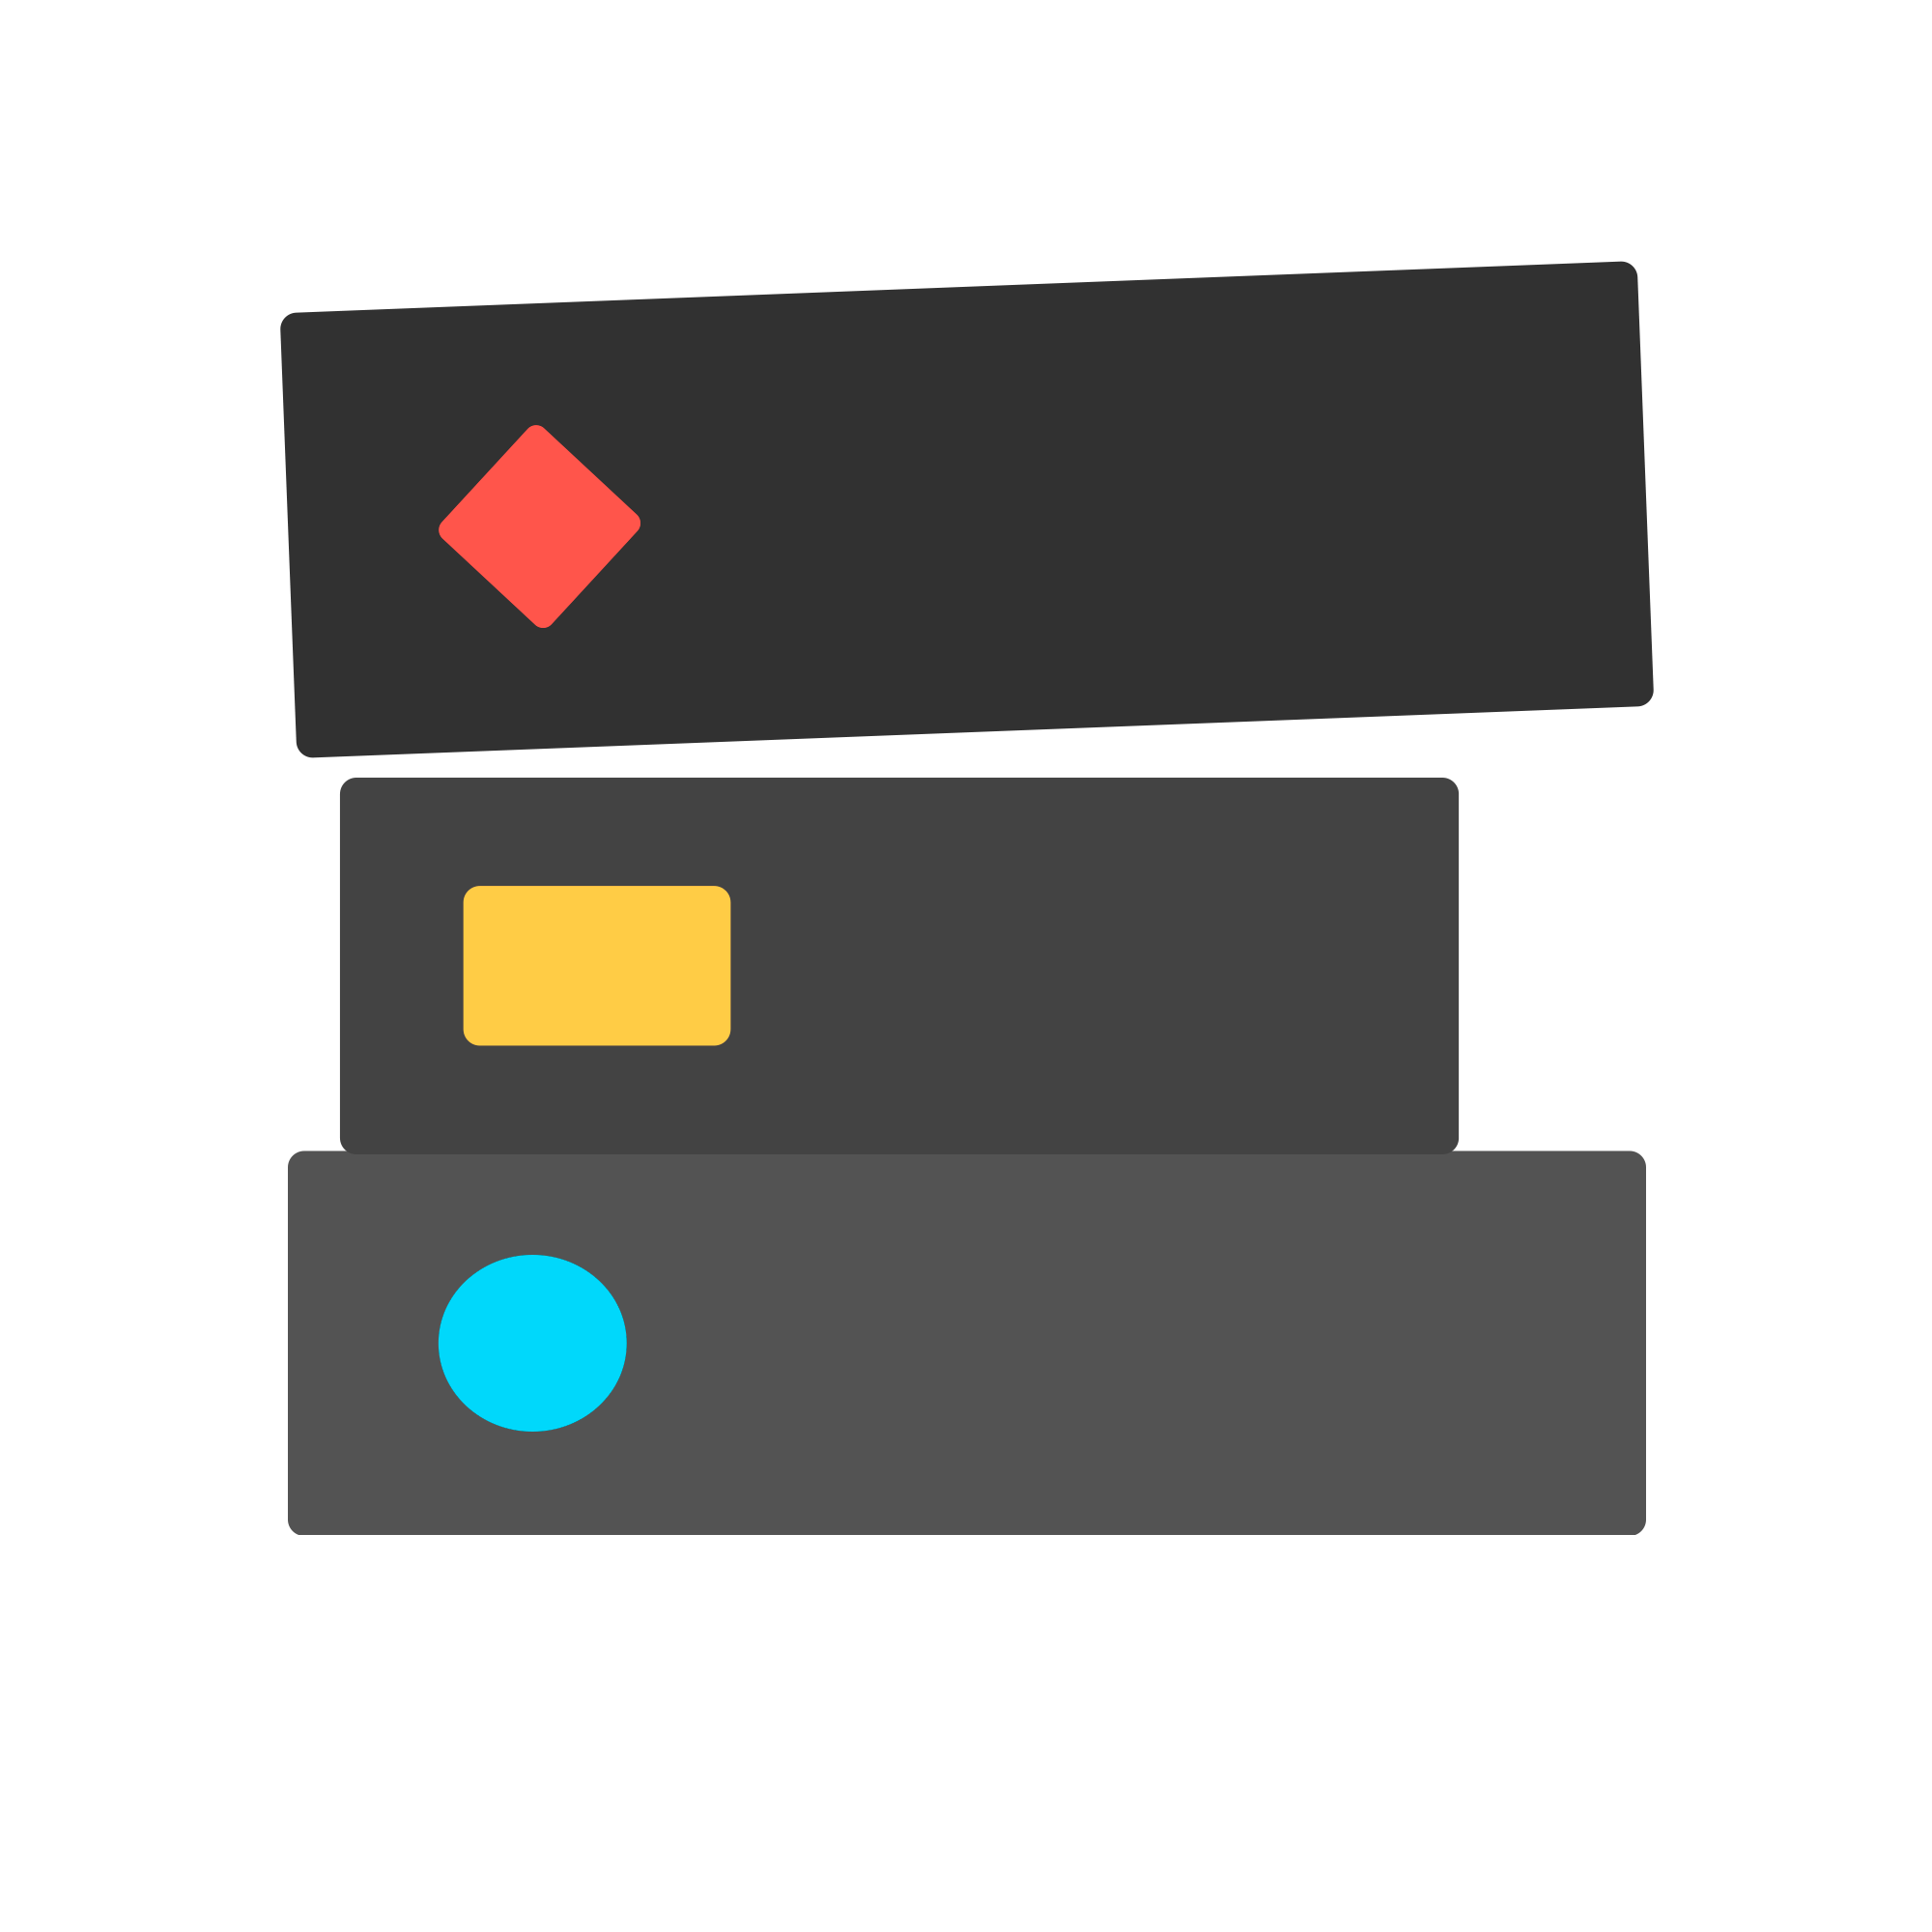
\includegraphics[width=0.5\textwidth]{img/DBCase_logo.png}
\end{figure}
%%
\section{Introducción}
DBCASE 2.0 surge como una actualización al proyecto DBCASE con la que se pretende dar un nuevo aspecto al diseño de la interfaz de usuario y continuar con la implementación de nuevas funcionalidades.\\

El programa está destinado principalmente al uso académico y por ello ha sido pensado como una herramienta didáctica que ayude al alumno en su proceso de aprendizaje, aunque también puede ser usada profesionalmente como una manera fácil y rápida de construir una base de datos relacional. Por ello la herramienta permite al usuario crear una base de datos funcional a partir de un diagrama sin necesidad de que conozca ningún lenguaje de programación de base de datos, lo que es perfecto para alumnos que se estén iniciando en la materia.\\

La herramienta está desarrollada íntegramente utilizado el lenguaje de programación Java.

%%
\subsection{Antecedentes}
El proyecto DBCase 2.0 es la continuación de dos proyectos anteriores.\\

\textbf{DBDT} de sistemas informáticos (2007/2008)\\
Autores del proyecto:
\begin{itemize}
    \item Alberto Milán Gutierrez.
    \item Miguel Martinez Segura
    \item Francisco Javier Cáceres González
    \item Profesora Directora: Yolanda García Ruiz
\end{itemize}

\textbf{DBCase} de sistemas informáticos (2008/2009)\\
Autores del proyecto:
\begin{itemize}
    \item Rodrigo Denis Cepeda Mateos
    \item Cristina Marco de Francisco
    \item Tello Serrano Gordillo
\end{itemize}
El proyecto servía como una herramienta bastante útil, pero que debido al paso de los años había quedado algo obsoleta. Sobre todo en lo que respecta a su interfaz gráfica.
%%
\subsection{Objetivos}
El principal objetivo del proyecto era rehabilitar la aplicación para su uso académico en las aulas, para lo cual era necesario satisfacer dos cuestiones.
\begin{itemize}
    \item Actualizar el diseño de la interfaz gráfica de la aplicación, haciéndola más usable y moderna.
    \item Corregir los posibles errores que arrastrase la aplicación desde versiones anteriores y continuar añadiendo funcionalidades nuevas.
\end{itemize}
